\documentclass[lettersize,journal]{IEEEtran}
\usepackage{amsmath,amsfonts}
\usepackage{algorithmic}
\usepackage{algorithm}
\usepackage{array}
\usepackage[caption=false,font=footnotesize]{subfig}
\usepackage{textcomp}
\usepackage{stfloats}
\usepackage{url}
\usepackage{verbatim}
\usepackage{graphicx}
\usepackage{cite}
\usepackage{float}

\usepackage{xcolor}
\usepackage{soul}

% --- CL float stabilization (minimal) ---
\setlength{\textfloatsep}{5pt}
\setlength{\floatsep}{5pt}
\setlength{\intextsep}{5pt}

\hyphenation{op-tical net-works semi-conduc-tor IEEE-Xplore}
% updated with editorial comments 8/9/2021

\begin{document}

\title{RF Feedback-based I/Q Imbalance Pre-Compensation for OFDM Systems}

\author{Jihoon~Lee and Jin~Kwan~Kim% <-this % stops a space
%\IEEEmembership{, Member,~IEEE}

\thanks{
J. Lee is with Satellite Communication Research Division, Electronics and Telecommunications Research Institute (ETRI), Daejeon 34129, Republic of Korea (e-mail: jihoonlee0104@etri.re.kr).

J. K. Kim (corresponding author) is an independent researcher, Taean, Chungcheongnam-do 32164, Republic of Korea (e-mail: tull00@hanyang.ac.kr).
}

%This work was supported by Institute for Information \& communications Technology Planning \& Evaluation (IITP) grant funded by the Korea government (KNPA) (No.2019-0-01291, LTE-based accurate positioning technique for emergency rescue).
%This work was in part supported by the research fund of Hanyang University.}
}

% The paper headers
%\markboth{Journal of \LaTeX\ Class Files,~Vol.~14, No.~8, August~2021}%
%{Shell \MakeLowercase{\textit{et al.}}: A Sample Article Using IEEEtran.cls for %IEEE Journals}

%\IEEEpubid{0000--0000/00\$00.00~\copyright~2021 IEEE}
% Remember, if you use this you must call \IEEEpubidadjcol in the second
% column for its text to clear the IEEEpubid mark.

\maketitle

\begin{abstract}
%In this paper, we propose an RF feedback-based predistortion scheme to mitigate I/Q imbalance in Orthogonal Frequency Division Multiplexing (OFDM) communication systems, in which gain and phase errors are estimated in real time using internal feedback from the RF signal.
%In this paper, we propose \hl{an RF feedback-based} predistortion scheme to mitigate I/Q imbalance in Orthogonal Frequency Division Multiplexing (OFDM) communication systems, \hl{in which} gain and phase errors are estimated \hl{obtained from} internal feedback from the RF signal \hl{rather than from pilot signals or a priori knowledge}.
In this paper, we propose an RF feedback-based predistortion scheme to mitigate I/Q imbalance in Orthogonal Frequency Division Multiplexing (OFDM) communication systems, in which gain and phase errors are \hl{estimated from internal RF feedback, without relying on} pilot signals or a priori knowledge.
%As a data-driven alternative, a Bidirectional Long Short-Term Memory (BLSTM)-based predistorter is also investigated, which learns the compensation mapping from training data using the estimated parameters as auxiliary inputs.
As a data-driven alternative, a Bidirectional Long Short-Term Memory (BLSTM)-based predistorter is also investigated, which \hl{uses the estimated parameters as auxiliary inputs to learn the compensation mapping from training data.}
%The simulation results show that both schemes achieve Error Vector Magnitude (EVM) and Bit Error Rate (BER) performance close to the ideal case under randomly varying I/Q imbalance.
The simulation results show that, \hl{under randomly varying I/Q imbalance,} both schemes achieve Error Vector Magnitude (EVM) and Bit Error Rate (BER) performance close to the ideal case \hl{without I/Q imbalance.}
\end{abstract}

\begin{IEEEkeywords}
I/Q imbalance, predistortion, deep learning, OFDM
\end{IEEEkeywords}

\section{Introduction}
\IEEEPARstart{W}{ith} the evolution from 5G New Radio (NR) to the emerging sixth generation (6G) wireless systems, there is an increasing demand for higher data rates, lower latency, and massive connectivity.
Both NR and emerging 6G systems adopt Orthogonal Frequency Division Multiplexing (OFDM) waveforms per recent 3GPP standards \cite{REF1, RP-25xxxx, RP-252912}.

OFDM offers several advantages, including high spectral efficiency and strong robustness against multi-path fading and Doppler effects \cite{Prasad}.
%OFDM enables efficient FFT-based signal processing and facilitates channel equalization in frequency-selective channels.
%Therefore, OFDM remains widely adopted in modern communication systems.
OFDM enables efficient FFT-based processing and channel equalization in frequency-selective channels, and therefore remains widely adopted.
However, OFDM systems are highly sensitive to impairments such as frequency offset, high 
Peak-to-Average Power Ratio (PAPR), Direct Current (DC) offset, I/Q imbalance, and phase noise \cite{REF4, REF5}.

Modern wireless systems demand highly integrated, low-cost receivers, making Zero Intermediate Frequency (zero-IF) receivers widely adopted \cite{REF6}.
%However, while baseband processing occurs in the digital domain, up/down-conversion is performed in the analog domain, where I/Q imbalance is inevitable due to gain and phase mismatches \cite{Razavi}.
However, up/down-conversion remains in the analog domain, where I/Q imbalance is inevitable due to gain and phase mismatches \cite{Razavi}.
As wireless systems move toward higher frequency bands and wider bandwidths in 6G, the impact of I/Q imbalance becomes increasingly severe due to heightened sensitivity of analog components to gain and phase mismatches at millimeter-wave frequencies.

Several research efforts have addressed I/Q imbalance \cite{REF7, REF8, REF9, Mirror_Image}.
However, \cite{REF7, REF8, REF9} require additional pilot signals, reducing spectral efficiency, and focus on post-compensation at the receiver.
Since post-compensation operates on the already-distorted received signal, the desired and image components must be separated after propagation, which is subject to channel estimation error and noise enhancement.
%In contrast, pre-compensation at the transmitter removes the impairment before the signal propagates through the channel, so that the receiver is not required to separate the desired and image components from the noisy received signal.
In contrast, pre-compensation at the transmitter removes the impairment before the signal propagates through the channel, so that the receiver is not required to separate the desired and image components from the \hl{distorted and noisy} received signal.
Reference \cite{Mirror_Image} addresses transmitter-side I/Q imbalance by exploiting the mirror interference structure, where paired subcarriers are used to pre-cancel the distortion at the transmitter.
However, this method assumes that the I/Q imbalance parameters are perfectly known a priori, which is difficult to guarantee in practice.
%When the compensation parameters deviate from the actual I/Q imbalance parameters, the mirror interference is incompletely canceled and manifests as residual self-interference, causing severe performance degradation with increasing parameter mismatch.
%When the compensation parameters deviate from the actual ones, the mirror interference is incompletely canceled and the residual self-interference degrades performance.
When the compensation parameters deviate from the actual ones, the mirror interference is incompletely canceled and the residual \hl{mirror interference} degrades performance.
The proposed scheme instead obtains these parameters from the internal RF feedback rather than relying on fixed a priori values.

Deep learning has also been applied to I/Q imbalance mitigation.
In~\cite{iqi_intel}, a machine learning-based transmitter mapper and receiver demapper are jointly trained to mitigate In-phase and Quadrature Imbalance (IQI) without estimating its coefficients and in \cite{dnn_otfs}, a DNN-based transceiver jointly performs channel training and IQI compensation.
In contrast, the proposed BLSTM-based scheme operates entirely at the transmitter and preserves the standard signal format, requiring no change at the receiver.

The main contributions of this paper are summarized as follows:

\begin{enumerate}
    %\item We propose an RF feedback-based predistortion scheme that estimates I/Q imbalance parameters in real time using internal RF feedback, without requiring pilot signals or a priori parameter knowledge.
    \item We propose an RF feedback-based predistortion scheme that obtains the I/Q imbalance parameters from internal RF feedback.
    Unlike \cite{REF7, REF8, REF9}, it requires no pilot signals, and unlike \cite{Mirror_Image}, it does not rely on fixed a priori values.
    
    \item As a data-driven alternative, we investigate a BLSTM-based predistorter that receives the estimated parameters as auxiliary inputs and learns the compensation mapping from 
    \hl{training} data.
    %\hl{It attains compensation performance equivalent to the analytical scheme at a higher computational cost, indicating that the estimated parameters alone are sufficient for a learned predistorter to reproduce the intended compensation.}
    It attains compensation performance equivalent to the analytical scheme \hl{at the expense of} a higher computational cost, indicating that the estimated parameters \hl{provide sufficient information} for a learned predistorter to reproduce the intended compensation.
\end{enumerate}

%The simulation results demonstrate that the proposed predistortion schemes improve the Bit Error Rate (BER) performance of the OFDM system under I/Q imbalance conditions.

\section{System model} \label{sec:system_model}

\subsection{OFDM System}
%In an OFDM system, a high-rate data stream is divided into multiple low-rate data streams.
The time-domain OFDM signal $x(t)$ is \cite{Prasad}

\begin{equation}
\label{eq1}
x(t) = \frac{1}{N}\sum_{n=0}^{N-1} X_{n} e^{j2\pi n\Delta ft}, \quad 0 \leq t < T
\end{equation}
where $N$ denotes the number of subcarriers, $X_n$ represents the data symbol on the $n$th subcarrier, $\Delta f =1/T$ is the subcarrier spacing and $T$ is OFDM symbol duration.
In (\ref{eq1}), the time-domain OFDM signal $x(t)$ can be expressed as a sum of in-phase signal $I(t)$ and quadrature signal $Q(t)$ $(x(t) = I(t) + jQ(t))$.

\subsection{I/Q Imbalance}
In the up-conversion process, in-phase and quadrature signals are mapped onto cosine and sine waves of Local Oscillator (LO), respectively.
In ideal up-conversion, the RF signal $s(t)$ is

\begin{equation}
\label{eq2}
s(t) = I(t) \cdot \cos (\omega_c t) + Q(t) \cdot \sin (\omega_c t), 
\end{equation}
where $\omega_c$ is the carrier frequency of the RF signal.

The signal with I/Q imbalance $\hat s(t)$ can be expressed as \cite{Razavi}

\begin{equation}
\label{eq3}
\begin{split}
\hat s(t) 
&= I(t) \left(1+\frac{\varepsilon}{2}\right) \cos \left(\omega_c t + \frac{\varphi}{2}\right) \\
&+ Q(t) \left(1-\frac{\varepsilon}{2}\right) \sin \left(\omega_c t - \frac{\varphi}{2}\right), 
\end{split}
\end{equation}
where $\varepsilon$ and $\varphi$ are the gain and phase errors of the transmitter LO, respectively.
This model assumes a frequency-independent (flat) I/Q imbalance, which is commonly used for narrowband OFDM systems.
In this model, $\varepsilon$ represents the amplitude mismatch between the I and Q branches, while $\varphi$ denotes the phase error relative to the ideal $90 ^ {\circ}$ phase difference between the LO signals.
In this paper, $\varepsilon$ and $\varphi$ are used to model only the transmitter-side I/Q imbalance.

\section{I/Q imbalance predistortion schemes}

\subsection{RF feedback-based predistortion of I/Q imbalance} \label{analytical_pred}

\begin{figure*}[!t]
\centering
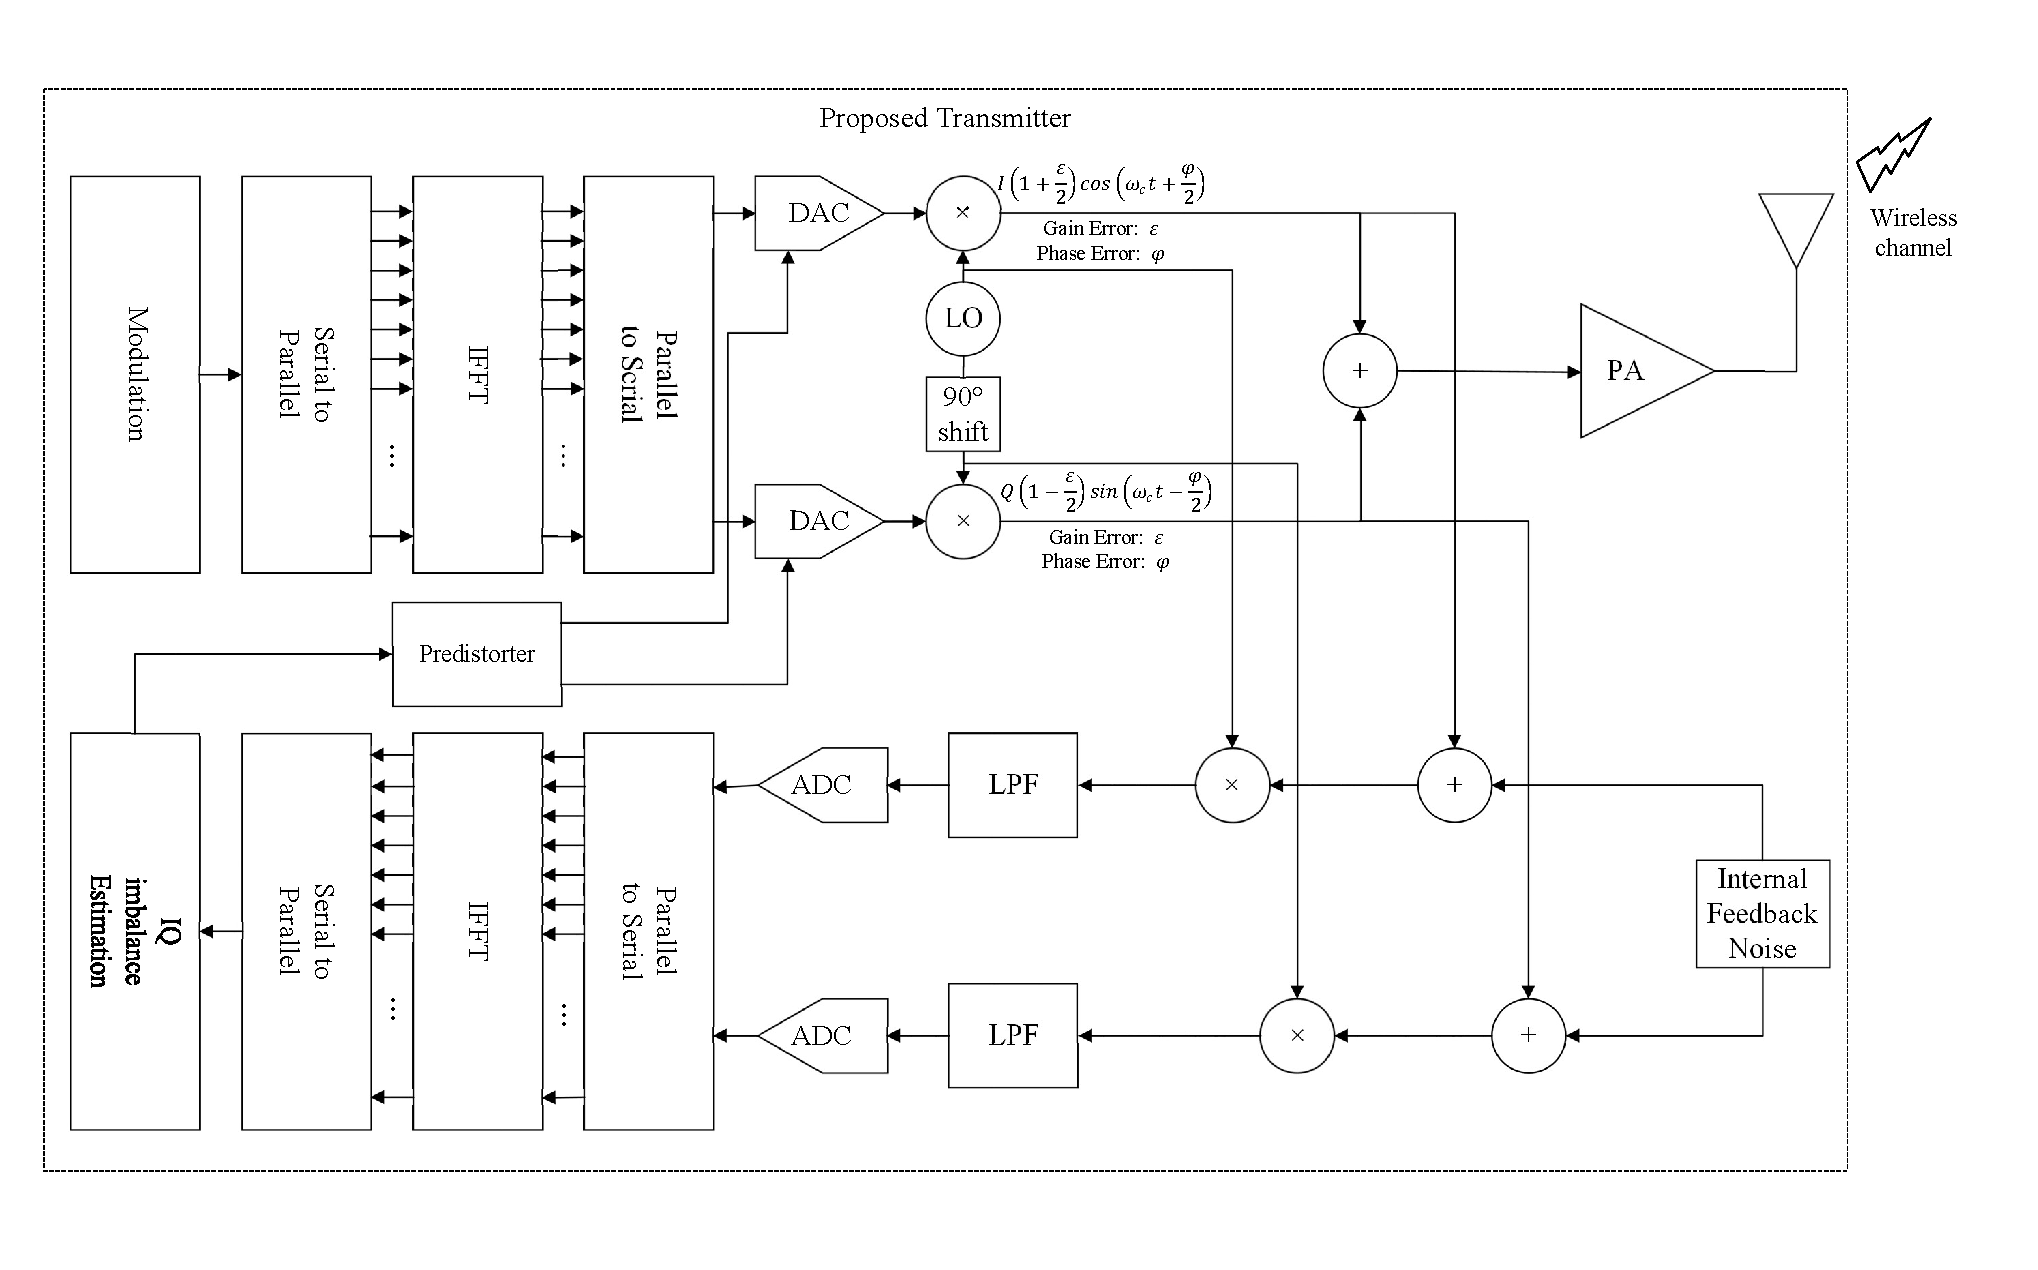
\includegraphics[width=0.8\textwidth]{Predistortor}
\caption{Block diagram of the proposed transmitter with RF feedback-based I/Q imbalance predistorter.}
\label{transmit}
\end{figure*}

Fig.~\ref{transmit} shows the block diagram of the proposed transmitter with an RF feedback-based I/Q imbalance predistorter, hereafter referred to as the analytical predistorter since it applies the analytically derived inverse of \eqref{eq3}.
%For clarity, the wireless channel and receiver are not shown, because the proposed scheme operates entirely at the transmitter side.
For clarity, the wireless channel and receiver are not modeled here, because the proposed scheme operates entirely at the transmitter side.
%The internal feedback path samples the up-converted RF signal before the power amplifier and performs down-conversion using the same LO employed for up-conversion within the same transmitter hardware.
%The internal feedback path samples the up-converted RF signal before the power amplifier and down-converts it using the same LO employed for up-conversion, \hl{so that both paths experience the same carrier frequency and phase.}
The internal feedback path samples the up-converted RF signal before the power amplifier and down-converts it using the same LO employed for up-conversion, so that \hl{any frequency or phase offset of the LO is common to both paths and thereby cancels out in the estimated I/Q imbalance parameters.}
This differs from receiver-side compensation schemes \cite{REF7, REF8, REF9}, which require synchronization between separate transmitter and receiver LOs.
In this work, the feedback chain is assumed to be noiseless and free from additional distortions to isolate the effect of I/Q imbalance.
During the estimation phase, the predistorter is bypassed so that the observed feedback signal reflects the I/Q imbalance alone.
Once the gain and phase errors are estimated, the switches direct the signal through the predistorter, which applies the estimated values until the next estimation phase.

The down-conversion signal $\tilde x(t)$ can be expressed as the sum of in-phase signal $\tilde I(t)$ and quadrature $\tilde Q(t)$ $(\tilde x(t) = \tilde I(t) + j \tilde Q(t))$.
Then, $\tilde I(t)$ and $\tilde Q(t)$ can be expressed as

\begin{equation}
\label{eq4}
\begin{split}
&\tilde I(t) 
= 2 \int_{0}^{t} \hat s(\tau) \left(1+\frac{\varepsilon}{2}\right) \cos \left(\omega_c \tau + \frac{\varphi}{2}\right) d\tau \\
&= I(t) \left(1+\frac{\varepsilon}{2}\right)^2 - Q(t) \left(1-\frac{\varepsilon^2}{4}\right) \sin \varphi,
\end{split}
\end{equation}

\begin{equation}
\label{eq5}
\begin{split}
&\tilde Q(t) 
= 2 \int_{0}^{t} \hat s(\tau) \left(1-\frac{\varepsilon}{2}\right) \sin \left(\omega_c \tau - \frac{\varphi}{2}\right) d\tau \\
&= Q(t) \left(1-\frac{\varepsilon}{2}\right)^2 - I(t) \left(1-\frac{\varepsilon^2}{4}\right) \sin \varphi,
\end{split}
\end{equation}

Taking a linear combination of \eqref{eq4} and \eqref{eq5}, where \eqref{eq4} and \eqref{eq5} are weighted by $I(t)$ and $-Q(t)$, respectively, eliminates the phase-dependent term $\sin \varphi$ and yields

\begin{equation}
    \label{eq6}
    \begin{split}
    I(t)\tilde{I}(t) - &Q(t)\tilde{Q}(t) \\ 
    &= I^2(t)\left(1+\frac{\varepsilon}{2}\right)^2- Q^2(t)\left(1-\frac{\varepsilon}{2}\right)^2
    \end{split}
\end{equation}

Rearranging \eqref{eq6}, the following equation with respect to $\varepsilon$ is obtained as

\begin{equation}
    \label{eq7}
    \begin{split}
    &(I^2(t) - Q^2(t))\varepsilon^2 + 4(I^2(t) + Q^2(t))\varepsilon\\
    & + 4[I^2(t)-Q^2(t) -I(t)\tilde{I}(t) + Q(t)\tilde{Q}(t)] = 0   
    \end{split}   
\end{equation}

The solution of \eqref{eq7} depends on the relationship between $|I(t)|$ and $|Q(t)|$.
When $|I(t)| = |Q(t)|$, the coefficient of quadratic term in \eqref{eq7} becomes zero, and the gain error $\varepsilon_T$ is directly obtained as

\begin{equation}
\label{eq8}
\varepsilon_T =
\frac{I(t) \tilde I(t) - Q(t) \tilde Q(t)}{I^2(t) + Q^2(t)}.
\end{equation}

On the other hand, for $|I(t)| \neq |Q(t)|$, \eqref{eq7} remains quadratic, yielding two candidate solutions as

\begin{equation}
\label{eq9}
\varepsilon_T =
\frac{-2[I^2(t) + Q^2(t)] \pm
2\sqrt{\Delta}}
{I^2(t) - Q^2(t)},
\end{equation}
where $\Delta = 4I^2(t)Q^2(t)+[I^2(t)-Q^2(t)][I(t) \tilde I(t) - Q(t) \tilde Q(t)]$.
From \eqref{eq7}, the sum of the two solutions always exceeds 4 in magnitude.
However, in \eqref{eq3}, the branch gains remain physically meaningful only for $|\varepsilon|<2$.
Since the two solutions cannot both satisfy this constraint, the one with the larger absolute value is discarded as spurious.
Accordingly, among the two candidate solutions, the one with the smaller absolute value is selected as the physically meaningful solution $\varepsilon_T$.

In \eqref{eq9}, the term $-2[I^2(t)+Q^2(t)]$ in the numerator is always negative, so taking the plus sign before $\sqrt{\Delta}$ always yields a numerator of smaller magnitude than taking the minus sign.
Since $|\varepsilon_T|$ is the ratio of the numerator and denominator magnitudes, the solution obtained with the plus sign always has the smaller absolute value, irrespective of the sign of the denominator in \eqref{eq9}.
\hl{In practice,} \eqref{eq8} \hl{is also used when $|I(t)| \approx |Q(t)|$ (within a small threshold), where the denominator of} \eqref{eq9} \hl{becomes small.}
Consequently, the gain error $\varepsilon_T$ can be summarized as

\begin{equation}
\label{eq10}
\varepsilon_T =
\begin{cases}
\dfrac{I(t)\tilde{I}(t)-Q(t)\tilde{Q}(t)}{I^2(t)+Q^2(t)}, &|I(t)|=|Q(t)|, \\[1.5em]
\dfrac{-2\left[I^2(t)+Q^2(t)\right]+2\sqrt{\Delta}}{I^2(t)-Q^2(t)},&|I(t)|\neq |Q(t)|,
\end{cases}
\end{equation}

Using the estimated gain error $\varepsilon_T$, the phase error $\varphi_T$ can be obtained from \eqref{eq4} or \eqref{eq5} as

\begin{equation}
\label{eq11}
\varphi_T =
\begin{cases}
\sin^{-1}\left(\dfrac{I(t)(1+\varepsilon_T/2)^2 - \tilde{I}(t)}{Q(t)(1-\varepsilon_T^2/4)}\right), & |Q(t)| \geq |I(t)|, \\[3ex]
\sin^{-1}\left(\dfrac{Q(t)(1-\varepsilon_T/2)^2 - \tilde{Q}(t)}{I(t)(1-\varepsilon_T^2/4)}\right), & |Q(t)| < |I(t)|,
\end{cases}
\end{equation}
where the expression with the larger denominator magnitude is selected to avoid numerical instability when either $|I(t)|$ or $|Q(t)|$ approaches zero.

%The predistorted signals $I_{PD}(t)$ and $Q_{PD}(t)$, obtained using $\varepsilon_T$ and $\varphi_T$ estimated from \eqref{eq10} and \eqref{eq11}, are given by
%\hl{The predistorter applies the inverse of} \eqref{eq3} \hl{using the estimated $\varepsilon_T$ and $\varphi_T$.
\hl{Using the estimated $\varepsilon_T$ and $\varphi_T$}, the predistorter applies the inverse of \eqref{eq3}, \hl{as derived below.}
Substituting the predistorted signals $I_{PD}(t)$ and $Q_{PD}(t)$ into \eqref{eq3} and matching the coefficients of $\cos \omega_c t$ and $\sin \omega_c t$ with those of the ideal RF signal in \eqref{eq2} yields

\begin{equation}
\label{pd_mat}
\begin{bmatrix} I(t) \\ Q(t) \end{bmatrix}
= \mathbf{M}(\varepsilon_T,\varphi_T)
\begin{bmatrix} I_{PD}(t) \\ Q_{PD}(t) \end{bmatrix},
\end{equation}

\begin{equation}
\label{pd_M}
\mathbf{M}(\varepsilon,\varphi) =
\begin{bmatrix}
\left(1+\frac{\varepsilon}{2}\right)\cos\frac{\varphi}{2} & -\left(1-\frac{\varepsilon}{2}\right)\sin\frac{\varphi}{2} \\[0.5em]
-\left(1+\frac{\varepsilon}{2}\right)\sin\frac{\varphi}{2} & \left(1-\frac{\varepsilon}{2}\right)\cos\frac{\varphi}{2}
\end{bmatrix}.
\end{equation}

Since $\det \mathbf{M} = (1-\varepsilon^2/4)\cos\varphi \neq 0$ within the practical range of $\varepsilon$ and $\varphi$, the predistorted signals are obtained as

\begin{equation}
\label{pd_IQ}
\begin{bmatrix} I_{PD}(t) \\[0.4em] Q_{PD}(t) \end{bmatrix}
= \frac{1}{\cos\varphi_T}
\begin{bmatrix}
\dfrac{I(t)\cos\frac{\varphi_T}{2} + Q(t)\sin\frac{\varphi_T}{2}}{1+\varepsilon_T/2} \\[1.1em]
\dfrac{I(t)\sin\frac{\varphi_T}{2} + Q(t)\cos\frac{\varphi_T}{2}}{1-\varepsilon_T/2}
\end{bmatrix}.
\end{equation}
The gain error scales each branch individually, whereas the phase error couples the two branches through the off-diagonal terms of \eqref{pd_M}.
%For $\varphi_T = 0$, \eqref{pd_IQ} reduces to the branch-wise gain correction $I_{PD} = I/(1+\varepsilon_T/2)$ and $Q_{PD} = Q/(1-\varepsilon_T/2)$.
%The observation matrix relating $[I(t)~Q(t)]^{\mathsf{T}}$ to $[\tilde I(t)~\tilde Q(t)]^{\mathsf{T}}$ in \eqref{eq4} and \eqref{eq5} is given by $\mathbf{M}^{\mathsf{T}}\mathbf{M}$, since the feedback path applies the same LO twice.

\subsection{Deep learning-based predistortion of I/Q imbalance} \label{deep_learn_pred}

%The predistorter in Section~\ref{analytical_pred} applies the analytically derived inverse of the imbalance model in \eqref{eq3}.
%As an alternative, this subsection investigates a data-driven predistorter that learns the compensation mapping from training data.
%Both schemes use the same estimated parameters; they differ in how the compensation is realized.
As an alternative to the analytically derived inverse in Section \ref{analytical_pred}, this subsection investigates a data-driven predistorter that learns the compensation mapping from training data.
\hl{Both schemes use the same estimated parameters and differ only in how the compensation is realized.}

%In this paper, we employ BLSTM as a deep learning-based approach for I/Q imbalance predistortion.
%Unlike traditional LSTM, BLSTM processes information bidirectionally, utilizing both past and future context \cite{REF10}.
\hl{We employ a BLSTM, which processes the input sequence bidirectionally and thus exploits both past and future context} \cite{REF10}.
 
\hl{The I/Q imbalance in} \eqref{eq3} \hl{is memoryless, in that the distortion at each time instant depends only on the instantaneous values of $I(t)$ and $Q(t)$ and the underlying $\varepsilon$ and $\varphi$.
Since the predistortion target depends on $\varepsilon$ and $\varphi$, the estimated parameters are provided to the network as auxiliary inputs so that the mapping is uniquely defined for a given input sequence.
Since the mapping is memoryless, a per-sample network would in principle suffice.
A sequence model is nevertheless adopted because the entire OFDM symbol is buffered at the transmitter in any case, and because sequence context becomes relevant once the impairment departs from the memoryless model in} \eqref{eq3}\hl{.
BLSTM-based sequence modeling has also been investigated for wideband RF power amplifier behavioral modeling and linearization} \cite{pa_blstm}.

%Each BLSTM input sequence consists of the \hl{$N$} time-domain samples of one OFDM symbol obtained after the IFFT and P/S conversion, \hl{together with the estimated $\varepsilon$ and $\varphi$ appended as two additional input features held constant over the sequence.
%Since the predistortion is applied to the baseband $I(t)$ and $Q(t)$ before up-conversion, where the two branches are still separate, each branch is affected only by its own gain and phase deviation in \eqref{eq3}.
%Therefore, the I and Q components are compensated by two independent BLSTM networks with identical structures.
As shown in \eqref{pd_IQ}, \hl{both predistorted components depend on $I(t)$ and $Q(t)$ through the phase error.
Each BLSTM input sequence therefore consists of the $N$ time-domain samples of $I(t)$ and $Q(t)$ for one OFDM symbol, obtained after the IFFT and P/S conversion, together with the estimated $\varepsilon$ and $\varphi$ appended as two additional input features held constant over the sequence.}

%These signals pass through both forward and backward BLSTM layers, which learn sequential features.
%The forward and backward hidden states, denoted by $\overrightarrow{h}_t$ and $\overleftarrow{h}_t$, are expressed as

%\begin{equation}
%\label{eq_lstm_for}
%\overrightarrow{h}_t = \mathrm{LSTM}_{\mathrm{forward}}(x_t,\overrightarrow{h}_{t-1}),
%\end{equation}

%\begin{equation}
%\label{eq_lstm_back}
%\overleftarrow{h}_t = \mathrm{LSTM}_{\mathrm{backward}}(x_t,\overleftarrow{h}_{t+1}).
%\end{equation}

%Then, the combined hidden state $h_t$, obtained by combining the forward and backward hidden states, can be expressed as

%\begin{equation}
%\label{eq_comb_ht}
%h_t = [\overrightarrow{h}_t,\overleftarrow{h}_t].
%\end{equation}

%The BLSTM architecture consists of forward and backward LSTM layers that process the input sequence in both temporal directions.
%The outputs from the two directions are combined to generate the compensated signal \cite{REF10, pa_blstm}.

%The BLSTM model is trained using pairs of the original transmit signal and its predistorted counterpart, where the target is generated by applying the inverse of the I/Q imbalance model in \eqref{eq3} with the corresponding $\varepsilon$ and $\varphi$.
The BLSTM model is trained using pairs of the original transmit signal and its predistorted counterpart, where the target is generated by applying \eqref{pd_IQ} \hl{with the corresponding $\varepsilon$ and $\varphi$}.
The trained network thus learns the predistortion mapping $P(\cdot)$ such that $H_{IQ}(P(x)) \approx x$, where $H_{IQ}(\cdot)$ denotes the I/Q imbalance in \eqref{eq3}.
The loss function $L$ is defined as the Mean Squared Error (MSE) and can be expressed as

\begin{equation}
\label{eq_loss_func}
L = \frac{1}{N} \sum_{i=1}^{N}(|I_{i,\mathrm{ref}}-I_{i,\mathrm{comp}}|^2+|Q_{i,\mathrm{ref}}-Q_{i,\mathrm{comp}}|^2),
\end{equation}
where \hl{the summation is taken over the $N$ samples of one OFDM symbol,} $I_{i,\mathrm{ref}}$ and $Q_{i,\mathrm{ref}}$ are the in-phase and quadrature components of the reference predistorted signal, while $I_{i,\mathrm{comp}}$ and $Q_{i,\mathrm{comp}}$ are the corresponding components of the predistorted signal generated by the network.
%The network parameters are optimized by minimizing \eqref{eq_loss_func} between the reference and network-generated predistorted signals.

%For I/Q imbalance predistortion, the use of BLSTM algorithm offers several advantages.
%Once trained over a range of I/Q imbalance parameters, BLSTM compensates each input sequence without requiring explicit parameter values, making it applicable under varying parameter conditions without retraining.
%\hl{Moreover, the data-driven mapping is not restricted to the specific analytical form assumed in} \eqref{eq3}, \hl{which may be advantageous when the actual impairment deviates from the idealized model.
%However, it requires a large training dataset and additional computational resources compared to conventional techniques.}
\hl{Compared with the analytical predistorter, the BLSTM-based scheme requires a large training dataset and substantially higher computational resources without providing a performance gain in the considered setting.}

In this paper, considering the system complexity and hardware limitations, the OFDM system is designed with an FFT size of $N=32$.
The proposed BLSTM model consists of an input layer, two BLSTM hidden layers, and an output layer.
The first and second BLSTM hidden layers contain 70 and 90 units, respectively.
%The first layer is intended to capture the sample-wise imbalance characteristics within an OFDM symbol, while the second layer models higher-order dependencies among the samples.
%This configuration provides a reasonable trade-off between compensation accuracy and computational complexity.
\hl{The layer sizes were determined empirically among several candidate configurations, providing a reasonable trade-off between compensation accuracy and computational complexity.}

To train the BLSTM model, the Root Mean Square Propagation (RMSProp) optimizer was used.
The batch size was set to 32, and training was conducted over 60 epochs.
\hl{The dataset used for model development consisted of a total of 100,000 OFDM symbols, which were split into training (80,000 symbols) and validation (20,000 symbols) sets at a ratio of 4:1, where the validation set is used to monitor convergence during training.}

\begin{figure}[!t]
\centering
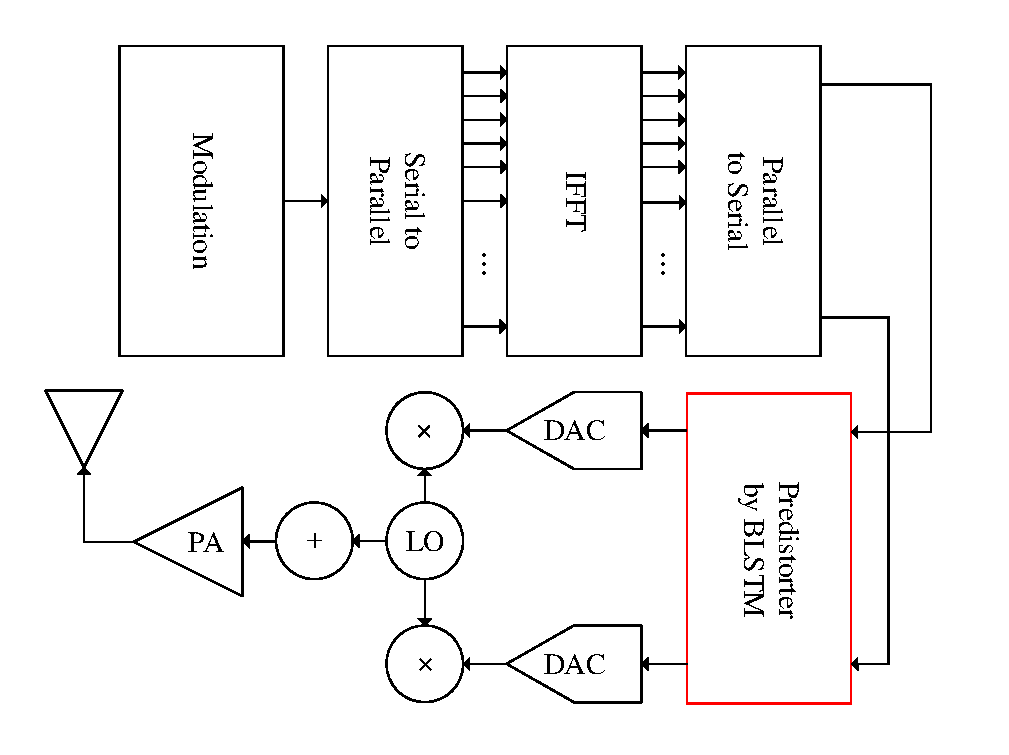
\includegraphics[width=0.8\linewidth]{transmit_blstm}
\caption{Block diagram of the proposed transmitter with BLSTM-based I/Q imbalance predistorter.}
\label{transmit_blstm}
\end{figure}

%Fig. \ref{transmit_blstm} shows the OFDM transmitter structure incorporating the proposed BLSTM-based predistorter for I/Q imbalance compensation.
%In Fig. \ref{transmit_blstm}, the BLSTM is applied after the Parallel-to-Serial (P/S) conversion. 
%During the BLSTM processing, the OFDM symbols are predistorted to mitigate the I/Q imbalance and then up-converted to the RF signal.
\hl{Fig.}~\ref{transmit_blstm} \hl{shows the OFDM transmitter incorporating the proposed BLSTM-based predistorter, where the predistortion is applied after the Parallel-to-Serial (P/S) conversion and the predistorted symbols are then up-converted to the RF signal.}

\section{Simulation Results} \label{simulation}

In this section, simulation results are presented.
The OFDM signal is modulated by Quadrature Phase Shift Keying (QPSK), and the number of subcarriers is set to 32.
As stated in Section~\ref{analytical_pred}, \hl{the feedback chain is assumed to be noiseless throughout the simulations, so that the estimated $\varepsilon_T$ and $\varphi_T$ coincide with the actual values.
The results therefore isolate the effect of the compensation itself and do not account for estimation error due to feedback noise or quantization.}

For BLSTM training, the input and target data are set to the original transmit signal and the corresponding predistorted signal \hl{computed using the $\varepsilon$ and $\varphi$ used to generate the training data}, respectively.
%The BLSTM training is performed independently for the I and Q components.
\hl{The two networks are trained separately, each with the same input.}
The I/Q imbalance is modeled by assuming a gain error $\varepsilon$ and a phase error $\varphi$ uniformly distributed in the ranges of $0.2 \sim 0.5$ and $2^\circ \sim 5^\circ$, respectively, while the training dataset in Section~\ref{deep_learn_pred} uses the wider ranges of $0.1 \le \varepsilon \le 0.6$ and $1^\circ \le \varphi \le 6^\circ$ to encompass the test range and thereby avoid extrapolation.
%Although $\varepsilon$ and $\varphi$ are modeled as static parameters in the analytical derivation, they may vary in practice due to temperature fluctuations, component aging, and signal-dependent effects.
%To evaluate the proposed schemes under randomly varying I/Q imbalance conditions, the gain and phase errors are resampled uniformly at random every 50 OFDM symbols, serving as a stress test regardless of the specific underlying mechanism.
\hl{Although $\varepsilon$ and $\varphi$ are static in the analytical derivation, they may vary in practice due to temperature fluctuations, component aging, and signal-dependent effects.
As a stress test, the gain and phase errors are resampled uniformly at random once per frame, which corresponds to every 50 OFDM symbols.
This interval is chosen as a simulation parameter to exercise the tracking capability rather than to represent a physical coherence time.
The estimation is performed once per frame so that the predistorter always operates with the current parameters.}
The test dataset, generated independently from the training and validation data, consists of 2,000 frames, each containing 50 OFDM symbols over which the gain and phase errors remain constant.

%The performance of the training model was evaluated using the MSE.
%On the test dataset, the proposed BLSTM-based predistortion model achieved an MSE of $1.2 \times 10^{-4}$, demonstrating stable compensation performance under the considered I/Q imbalance conditions.
On the test dataset, the BLSTM-based predistortion model achieved an MSE of $1.2 \times 10^{-4}$, \hl{indicating} stable compensation under the considered I/Q imbalance conditions.

For the conventional mirror image method~\cite{Mirror_Image}, which assumes a priori knowledge of the I/Q imbalance parameters, the compensation is performed using fixed mid-range values of $\varepsilon_c = 0.35$ and $\varphi_c = 3.5^\circ$, consistent with the assumption in~\cite{Mirror_Image} that these parameters are known and time-invariant.
%Although this random variation does not explicitly capture physical drift mechanisms, it provides a controlled scenario exposing the mismatch between such fixed values and the randomly varying I/Q imbalance, under which the proposed RF feedback-based and BLSTM-based schemes continue to compensate for the varying I/Q imbalance whereas~\cite{Mirror_Image} inevitably suffers from mismatch.
\hl{This provides a controlled scenario exposing the mismatch between such fixed values and the randomly varying I/Q imbalance. In this scenario,} \cite{Mirror_Image} \hl{suffers from parameter mismatch, whereas the proposed schemes operate with the current estimates and follow the variation.}
 
%\subsection{Signal constellation under I/Q imbalance}

%\begin{figure}[!t]
%\centering
%\subfloat[With IQ imbalance]{\label{const_iq_imbal}
%    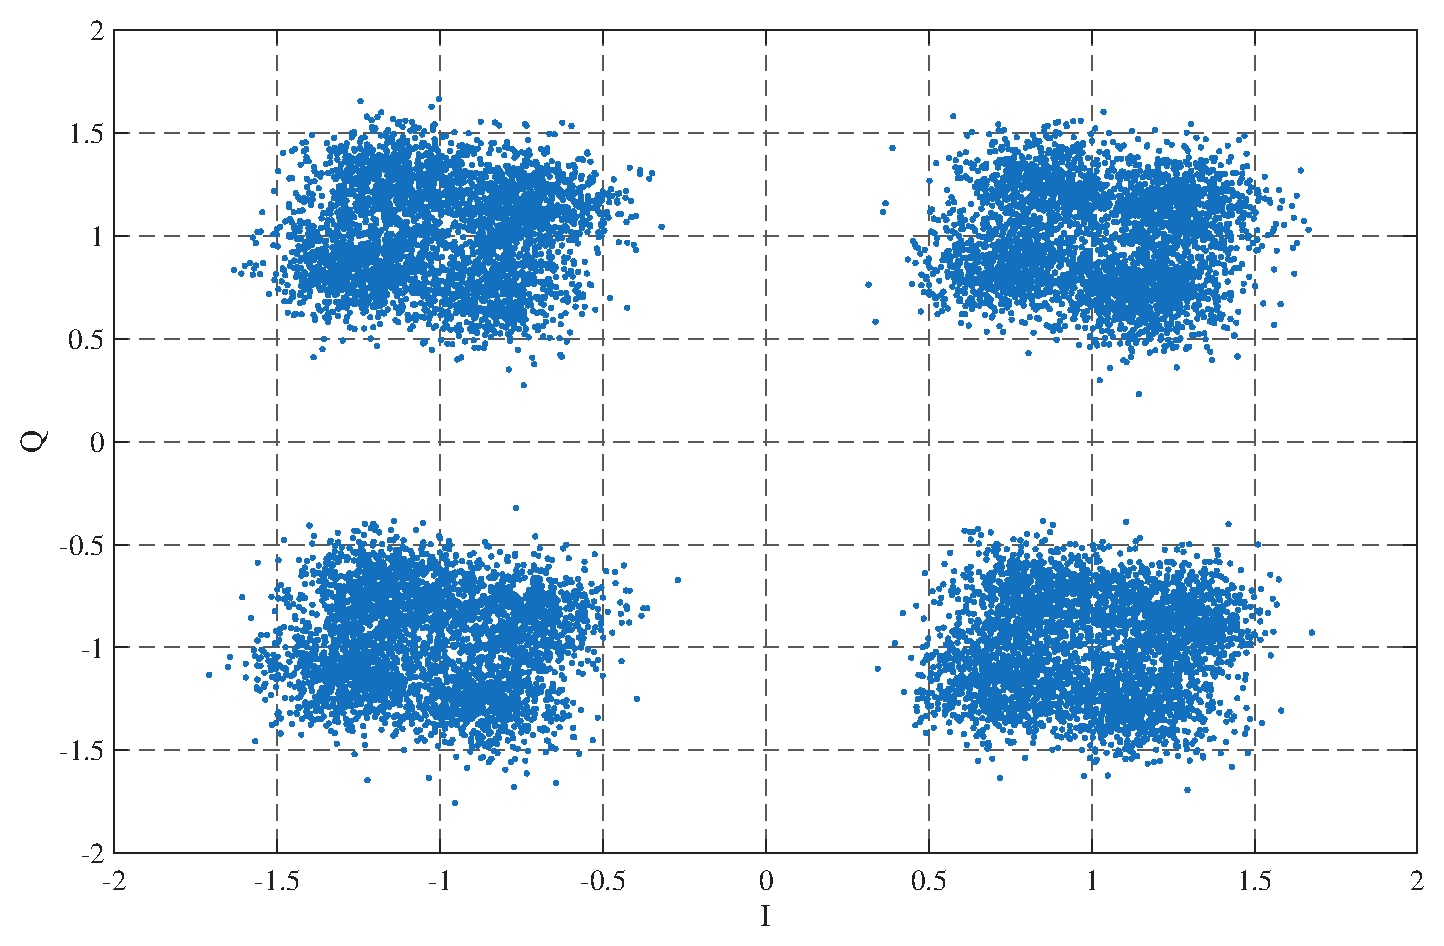
\includegraphics[width=0.75\linewidth]{const_iq_imbal}}
%\vfill
%\subfloat[After RF feedback-based predistortion]{\label{const_rf_pred}
%    \includegraphics[width=0.75\linewidth]{const_rf_pred}}
%    \vfill
%\subfloat[After BLSTM predistortion]{\label{const_blstm}
%    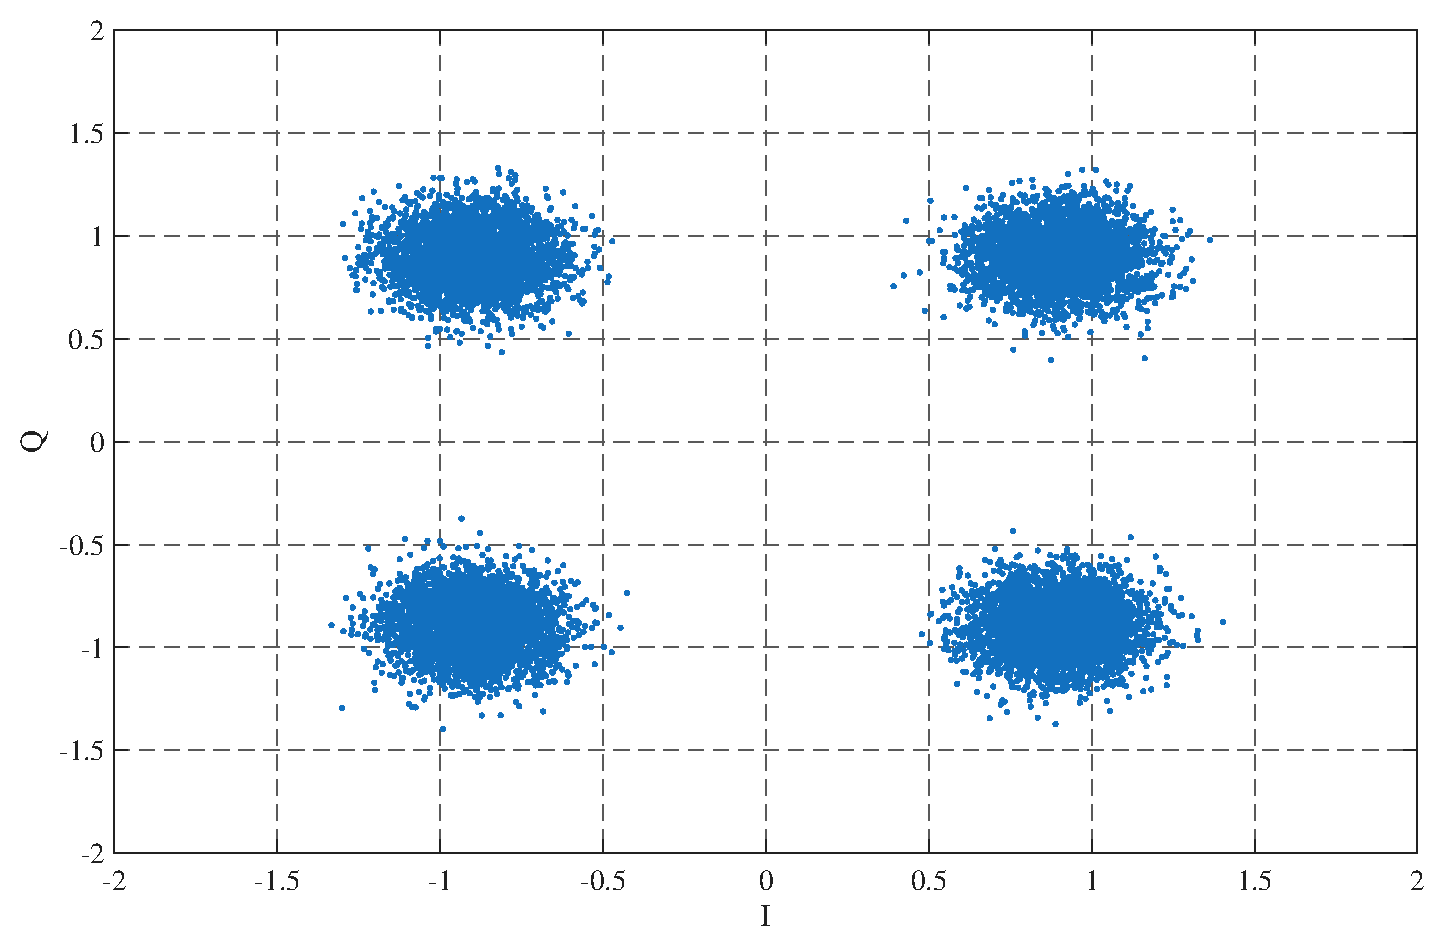
\includegraphics[width=0.75\linewidth]{const_blstm}}
%\caption{Signal constellations in AWGN at $E_b/N_0 = 15$ dB with $\varepsilon = 0.3$ and $\varphi = 5^\circ$.}
%\label{fig:const}
%\end{figure}

%Fig. \ref{fig:const} shows signal constellations in AWGN at $E_b/N_0 = 15$ dB with $\varepsilon = 0.3$ and $\varphi = 5^\circ$.
%In Fig.~\ref{fig:const}\subref{const_iq_imbal}, I/Q imbalance causes constellation dispersion, rotation, and the formation of multiple distinct clusters.
%This pattern arises because I/Q imbalance is modeled using discrete amplitude and phase error parameters, unlike random RF impairments such as phase noise.
%After RF feedback-based predistortion (Fig.~\ref{fig:const}\subref{const_rf_pred}) and BLSTM predistortion (Fig.~\ref{fig:const}\subref{const_blstm}), the constellation clouds are significantly reduced, demonstrating that both proposed schemes effectively compensate for the I/Q imbalance.

\subsection{Error Vector Magnitude (EVM) performance}

\begin{figure}[!t]
    \centering
    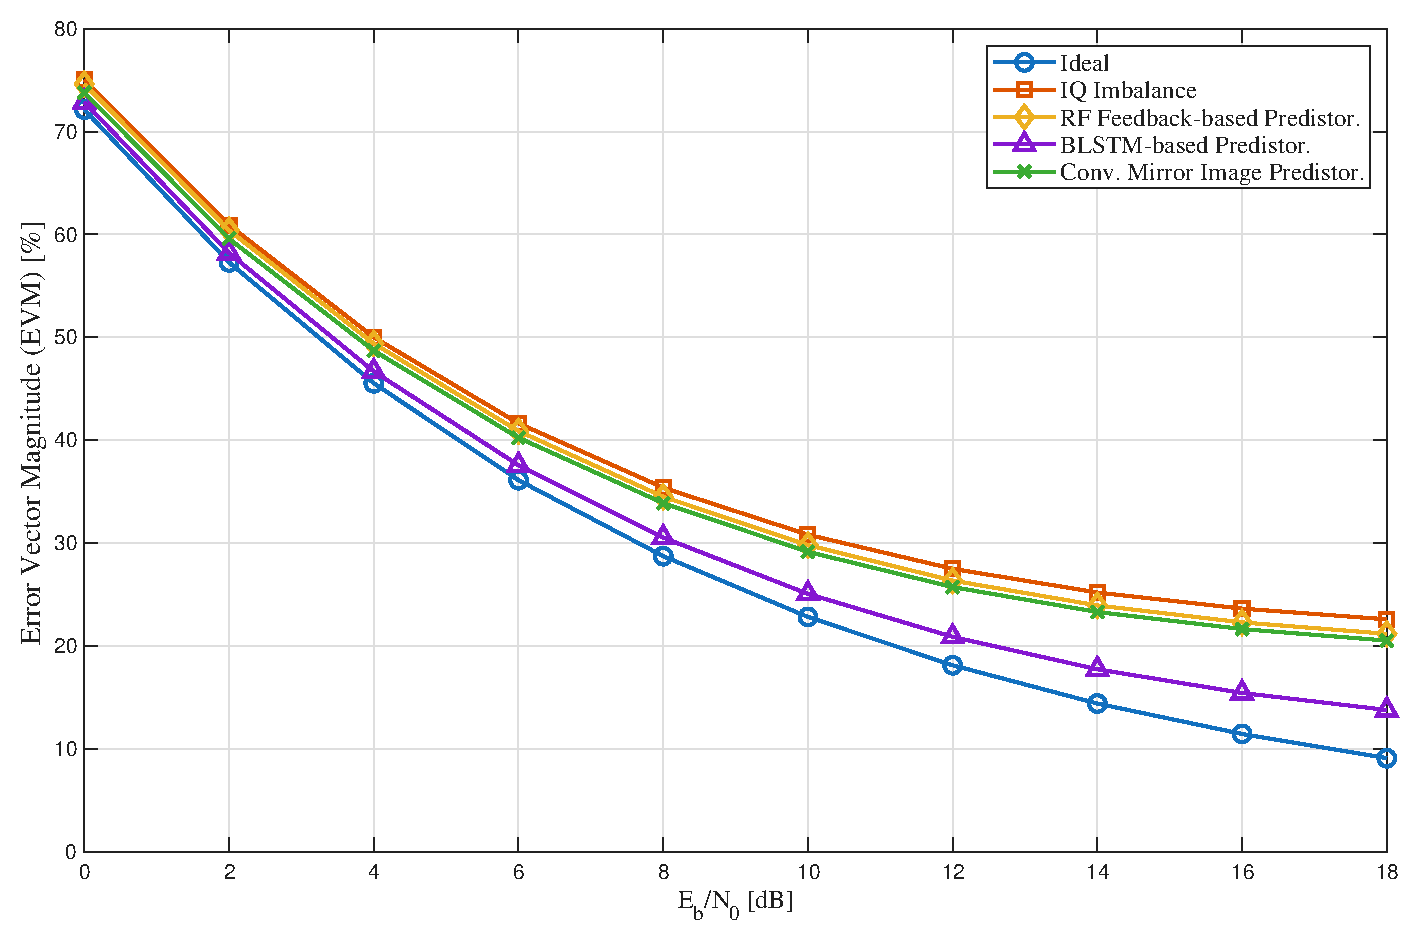
\includegraphics[width=0.8\linewidth]{evm}
    \caption{EVM performance comparison under I/Q imbalance in an AWGN channel.}
    \label{evm}
\end{figure}

Fig.~\ref{evm} shows the Error Vector Magnitude (EVM) performance of the two proposed predistortion schemes in an AWGN channel.
For comparison, the results for the uncompensated case and the ideal case (no I/Q imbalance) are also plotted.

At an EVM of 15\%, both the RF feedback-based and BLSTM-based schemes achieve approximately 2.7~dB improvement over the uncompensated case and 1.6~dB over the conventional mirror image method~\cite{Mirror_Image}, and %their EVM curves closely follow the ideal case across the entire $E_b/N_0$ range.
\hl{their EVM curves are indistinguishable from the ideal case across the entire $E_b/N_0$ range}.
\hl{The two schemes yield nearly identical performance, confirming that the BLSTM successfully learns the analytical predistortion mapping it is trained to reproduce.}
In contrast, \cite{Mirror_Image} attains only 1.1~dB improvement, as its fixed a priori parameters cannot follow the randomly varying I/Q imbalance.

\subsection{BER performance}

\begin{figure}[!t]
    \centering
    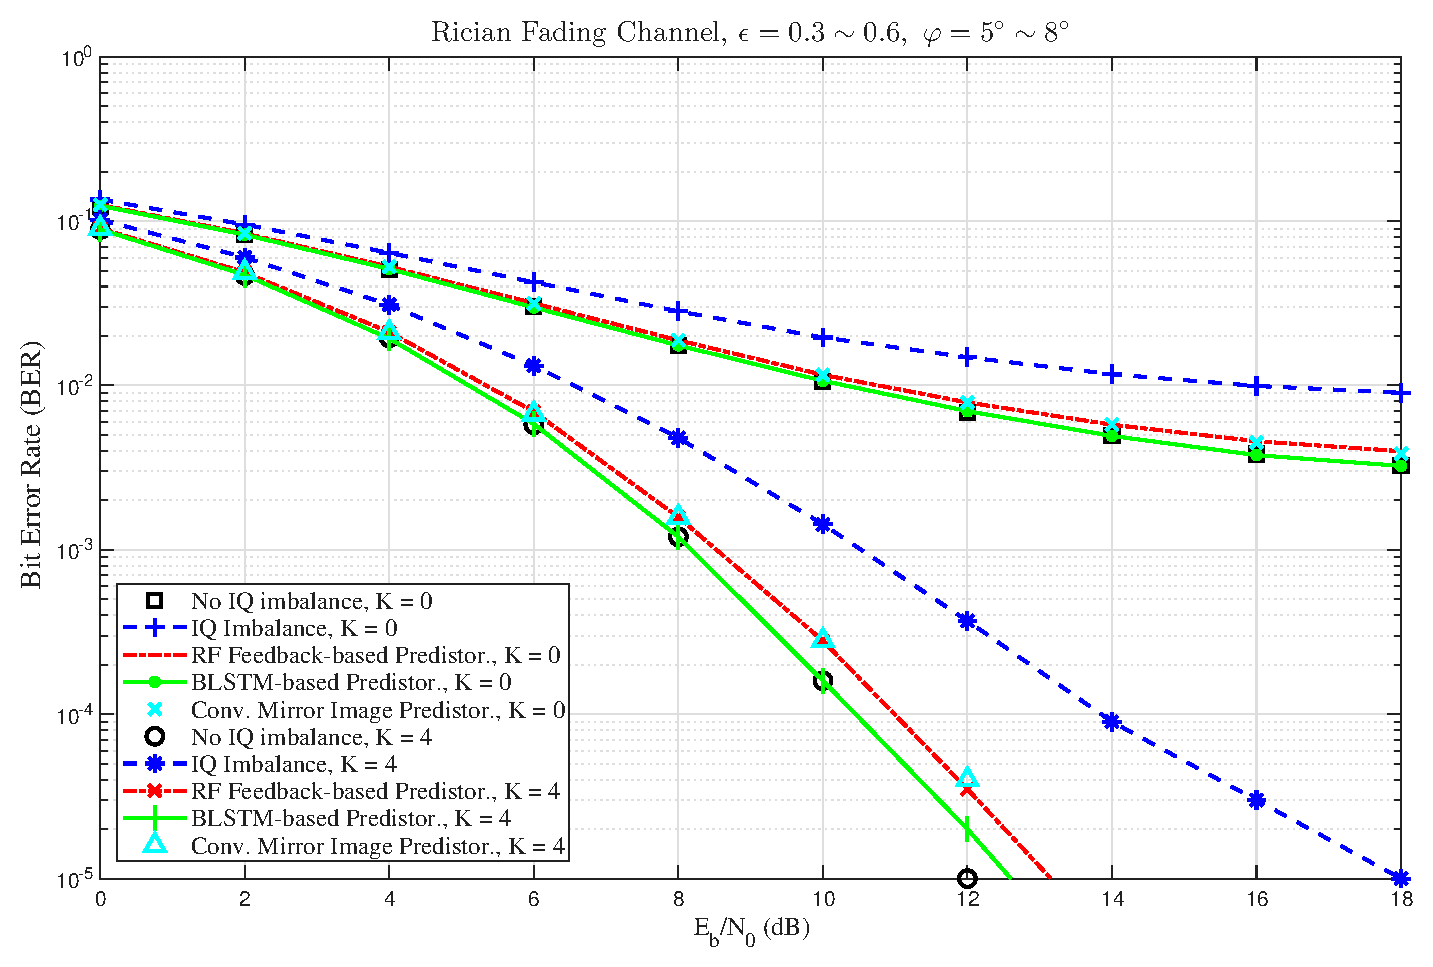
\includegraphics[width=0.8\linewidth]{ber}
    \caption{BER performance with and without I/Q imbalance predistortion over a Rician fading channel.}
    \label{ber}
\end{figure}

%Fig.~\ref{ber} shows the BER performance of the two proposed predistortion schemes in a Rician channel with $K$-factors of 8 and 20.
%For comparison, the results for the uncompensated case and the ideal case (no I/Q imbalance) are also plotted.
Fig.~\ref{ber} shows the BER performance of the two proposed predistortion schemes in a Rician channel with $K$-factors of 8 and 20, together with the uncompensated and ideal cases \hl{(no I/Q imbalance)}.
For $K = 8$ at a BER of $10^{-3}$, both proposed schemes achieve approximately 0.4~dB improvement over the uncompensated case, while the conventional mirror image method \cite{Mirror_Image} achieves about 0.2~dB.
For $K = 20$ at a BER of $10^{-5}$, the corresponding improvements are approximately 0.5~dB for the proposed schemes and 0.2~dB for \cite{Mirror_Image}.
In both channel conditions, the BER curves of the proposed schemes closely follow the ideal case, whereas \cite{Mirror_Image} exhibits a residual gap of about 0.2$\sim$0.3~dB caused by the mismatch between its fixed a priori parameters and the randomly varying I/Q imbalance.
Note that when identical parameters are available, the proposed RF feedback-based scheme and~\cite{Mirror_Image} realize equivalent compensation, so that the observed gap originates from the parameter mismatch rather than from the compensation structure itself.

%These results confirm that both proposed predistortion schemes effectively mitigate randomly varying I/Q imbalance under the considered scenario, achieving BER performance close to the ideal case.

\section{Conclusion}

This paper proposed \hl{an RF feedback-based} predistortion scheme for I/Q imbalance mitigation in OFDM systems.
Unlike \cite{REF7, REF8, REF9}, \hl{it requires} no pilot signals, and unlike \cite{Mirror_Image}, \hl{it obtains the imbalance parameters from the internal RF
feedback rather than relying on fixed a priori values.}
\hl{A BLSTM-based predistorter was also investigated as a data-driven alternative using the estimated parameters as auxiliary inputs.}

%Simulation results show that both schemes achieve EVM and BER performance close to the ideal case under randomly varying I/Q imbalance, whereas the conventional mirror image method \cite{Mirror_Image} exhibits a residual gap due to parameter mismatch.
%Although the BLSTM-based scheme does not outperform the analytical one in the considered setting, its model-agnostic nature may be advantageous under impairments that deviate from the idealized model, which remains as future work.
Simulation results \hl{show that both schemes achieve EVM and BER performance close to the ideal case under randomly varying I/Q imbalance, whereas the conventional mirror image method} \cite{Mirror_Image} \hl{exhibits a residual gap due to parameter mismatch.}

%\section*{Acknowledgments}
%This should be a simple paragraph before the References to thank those %individuals and institutions who have supported your work on this article.

% \textit{et al.}

\begin{thebibliography}{1}
\bibliographystyle{IEEEtran}

\bibitem{REF1}
3GPP TS 38.211, \emph{NR; Physical channels and modulation}, V19.4.0, Release 19, 3rd Generation Partnership Project, Sophia Antipolis, France, Jun. 2026.

\bibitem{RP-25xxxx}
3GPP TSG RAN meeting \#109, {\it{Status Report to TSG}}. Beijing, China, Sep. 2025.

\bibitem{RP-252912}
3GPP TSG RAN meeting \#109, {\it{Study on 6G Radio}}. Beijing, China, Sep. 2025.

\bibitem{Prasad}
R. Prasad, {\it{OFDM for wireless communications systems}}, Norwood, MA, USA: Artech House, 2004.

\bibitem{REF4}
S. Woo, D. Lee, K. Kim, Y. Hur, C. Lee, and J. Laskar, ``Combined effects of RF impairments in the future IEEE 802.11n WLAN systems,'' in \textit{Proc. IEEE VTC-SPRING}, Stockholm, Sweden, 2005, pp. 1346--1349.

\bibitem{REF5}
H. Ryu, Y. S. Li, and J. Park, ``Nonlinear analysis of the phase noise in the OFDM communication system,'' \textit{IEEE Trans. Consumer Electron.}, vol. 50, no. 1, pp. 54--63, Feb. 2004.

\bibitem{REF6}
A. A. Abidi, ``Direct-conversion radio transceivers for digital communications,'' \textit{IEEE Journal of Solid-State Circuits}, vol. 30, no. 12, pp. 1399--1410, Dec. 1995.

\bibitem{Razavi}
B. Razavi, {\it{RF Microelectronics}}, Upper Saddle River, NJ, USA: Prentice Hall, 1998.

\bibitem{REF7}
A. Schuchert, R. Hasholzner, and P. Antonie, ``A novel IQ imbalance compensation scheme for the reception of OFDM signals,'' \textit{IEEE Trans. Consumer Electron.}, vol. 47, no. 3, pp. 313--318, Aug. 2001.

\bibitem{REF8}
L. Anttila, M. Valkama, and M. Renfors, ``Blind Compensation of Frequency-Selective I/Q Imbalances in Quadrature Radio Receivers: Circularity-Based Approach,'' in \textit{Proc. IEEE ICASSP}, Honolulu, USA, 2007, pp. 245--248.

\bibitem{REF9}
A. Kiayani, L. Anttila, Y. Zou, and M. Valkama, ``Advanced Receiver Design for Mitigating Multiple RF Impairments in OFDM Systems: Algorithms and RF Measurements,'' \textit{Journal of Electrical and Computer Engineer.}, vol. 2012, no. 3, pp. 1--16, Jan. 2012.

\bibitem{Mirror_Image}
Y. Yuda, T. Kimura, S. Maki, and A. Nishio, ``Compensation of TX IQ imbalance in wideband OFDM systems,'' \textit{IEICE Commun. Express}, vol. 14, no. 8, pp. 301--304, Aug. 2025.

\bibitem{iqi_intel}
A. A. Boulogeorgos and A. Alexiou, ``Training Terahertz Wireless Systems to Battle I/Q Imbalance,'' in \textit{Proc. 2023 Intern. Balkan Conf. on Commun. and Network. (BalkanCom)}, İstanbul, Turkiye, 2023. DOI: 10.1109/BalkanCom58402.2023.10167934.

\bibitem{dnn_otfs}
A. Naikoti and A. Chockalingam, ``A DNN-based OTFS Transceiver with Delay-Doppler Channel Training and IQI Compensation,'' in \textit{Proc. 2021 IEEE 32nd Annual Intern. Symp. on Person., Indoor and Mobile Radio Commun. (PIMRC)}, Helsinki, Finland, 2021. DOI: 10.1109/PIMRC50174.2021.9569634.

\bibitem{REF10}
Y. Zhu, C. Gong, J. Luo, M. Jin, X. Jin, and Z. Xu, ``Indoor Non-Line of Sight Visible Light Communication with a Bi-LSTM Neural Network,'' in \textit{Proc. 2020 IEEE Intern. Conf. on Commun. Workshops (ICC Workshops)}, Dublin, Ireland, 2020, pp. 1--6.

%\bibitem{REF11}
%Md. A. I. Sunny, M. M. S. Maswood, and A. G. Alharbi, ``Deep learning-based stock price prediction using LSTM and bi-directional LSTM model,'' in \textit{Proc. 2020 2nd Novel Intelligent and Leading Emerging Sciences Conference (NILES)}, Giza, Egypt, 2020, pp. 87--92.

%\bibitem{REF12}
%Y. Imrana, Y. Xiang, L. Ali, and Z. Abdul-Rauf, ``A bidirectional LSTM deep learning approach for intrusion detection,'' \textit{Expert Syst. Appl.}, vol. 185, no. 8, Dec. 2021.

\bibitem{pa_blstm}
J. Sun, W. Shi, Z. Yang, J. Yang, and G. Gui, ``Behavioral Modeling and Linearization of Wideband RF Power Amplifiers Using BiLSTM Networks for 5G Wireless Systems,'' \textit{IEEE Trans. Veh. Technol.}, vol. 68, no. 11, pp. 10348--10356, Nov. 2019. DOI: 10.1109/TVT.2019.2925562.

\end{thebibliography}

\vfill

\end{document}